% -*- mode: latex; mode: outline-minor -*-
% Title:  tutorial
%
% Doc: /home/greg/usr/papers/lqns-tutorial/tutorial.tex
% Original Author:     Greg Franks <greg@sce.carleton.ca>
% Created:             Thu May 13 2004
%
% ------------------------------------------------------------------------
% $Id$
% ------------------------------------------------------------------------

\documentclass[11pt]{article}
\usepackage{times}
\usepackage{graphicx,dcolumn,verbatim,subfig,makeidx,color}
\usepackage{listings}
\usepackage[total={6.5in,8.7in}]{geometry}
\usepackage{hyperref}
\newcolumntype{d}[1]{D{.}{.}{#1}}
\newcommand{\parameter}[1]{\texttt{#1}\index{#1@\texttt{#1}}}
\makeindex

% Some useful definitions...
\setcounter{secnumdepth}{2}

\begin{document}
\lstdefinelanguage{LQN}{
  basicstyle=\ttfamily,
  keywords={G,P,U,T,E,A,R,C,p,g,t,s,c,f,y,z,u,F,-1,->,\#pragma},
  classoffset=1,
  morekeywords={<param>,<proc-id>,<group-id>,<task-id>,<entry-id>,<activity-id>,<sched>,<opt-mult>,<opt-cap>,<opt-pri>,<opt-grp>,<opt-think-time>,<opt-obs>,<opt-repl>,<value>,<expression>,<entry-list>,<activity-list>,<expression-list>,<real>,<int>,<string>},
  keywordstyle=\itshape,
  classoffset=0,
  alsoletter={-1<>},
  sensitive=true,
  morecomment=[l]{\# },
  morestring=[b]'',
  index={pragma}
}
\title{Tutorial Introduction to Layered Modeling of Software Performance}
\bibliographystyle{plainurl}
\author{Murray Woodside \and Greg Franks}
\date{Department of Systems and Computer Engineering\\
  Carleton University\\
  Ottawa ON K1S~5B6\\
  \texttt{\{cmw,greg\}@sce.carleton.ca}\\[1cm]
  \today}
\maketitle
\clearpage
\tableofcontents
\clearpage

\section{Introduction}

This note introduces the conceptual basis of layered queueing networks (LQNs) as a
performance model for software systems, and then leads the reader through the features provided by
the LQML modeling language. Layered queueing is an elegant compact notation for Extended
Queueing Networks, which incorporates a number of features which are common in software
systems (and other kinds of systems too). The central feature is a kind of structured ``simultaneous
resource possession''\index{simultaneous resource possession}, common in layered and client-server\index{client-server} architectures, which gives it the name
Layered Queueing\index{layered queueing}.

There is also a User Manual for the LQNS solver and LQSIM simulator, and a thesis~\cite{THESIS:franks-99} and
more recent technical paper~\cite{IEEESE:franks-2009-ieeese-lqn} which summarize the underlying mathematics; these and other
materials can be found on the \href{http://layeredqueues.org}{layeredqueues.org} web site, and on the LQNS page at
\url{www.sce.carleton.ca/rads/lqns}.

\section{Concepts}
\label{sec:concept}

Performance\index{performance}, in the sense of response times\index{response time} and throughputs\index{throughput}, is determined by how the
system's operations use its resources\index{resource}. While a resource is in use it is busy, and other requests for it
must wait, as determined by a queueing discipline. Ordinary queueing network (QN)\index{QN}\index{queueing network} performance
models are directly applicable to systems in which each operation requires only a single resource,
such as a CPU or disk; extended queueing networks (EQNs)\index{EQN} are needed for simultaneous resources\index{resource!simultaneous}.

Software systems often have software servers\index{server!software}\index{software server} that also have a queue\index{queue} of requests. When a
request is accepted by the software server process, the process must then request and wait for the
CPU. When it has the CPU, the operation can be executed and a reply returned for the request. This
is ``simultaneous resource possession''\index{simultaneous resource possession} with two layers of resources, the software server and the
CPU. The service time\index{service time} of the CPU is the host demand\index{host!demand}\index{demand} of the operation; the service time of the task
includes the waiting for the CPU as well, possibly waiting for several
``slices''\index{slice} of CPU time\index{CPU time}.

We consider layered systems (software systems, and other kinds of
systems too) that are made up of servers (and other resources which we
will model as servers); the generic term we will use for these
entities is ``task''\index{task}. A server is either a pure server\index{server!pure}, which executes
operations on command (for instance a processor), or a more complex
logical bundle of operations, which include the use of lower layer
services. Such a bundle of operations may be implemented as a software
server\index{server!software}.

\begin{figure}[h]
  \centering
  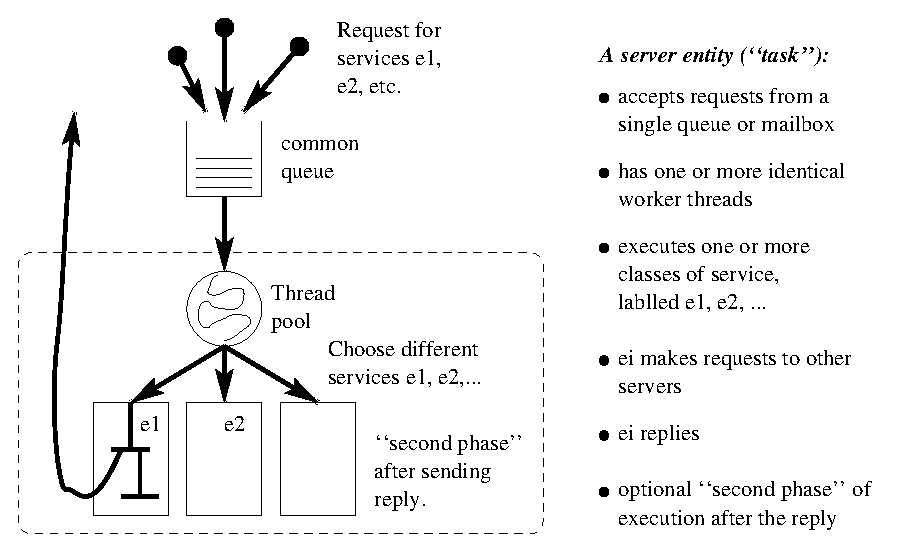
\includegraphics[height=3.25in]{model/elements.eps}
  \caption{The elements of a software server, including multiple
  threads, multiple entries, and second phases, which are all
  optional.} 
  \label{fig:elements}
\end{figure}

Figure~\ref{fig:elements} illustrates the elements of a software\index{server!sofware}
server, as they might be implemented in a software process. The
threads\index{threads} are servers to the queue, and the requests\index{requests} take the form of
interprocess messages\index{messages!interprocess} (remote procedure calls\index{remote procedure call}, or the semantic
equivalent), and the entries\index{entry} describe or define the classes of service\index{service!classes}
which can be given. The assumption in this theory is that each thread
has the capability of executing any entry.  The execution of the entry
can follow any sequence of operations, and can include any number of
nested requests or calls\index{requests!nested} to other servers. Calls to internal services
of the server are assumed to be included in the entry, so all calls
are to other servers. A canonical sequence of operations is the
first-phase/second phase sequence shown by the heavy line in the
figure, with the reply\index{reply} sent after the first phase\index{phase}. Software servers\index{server!software}
often send the reply as early as possible, and complete some
operations later (e.g. database commits).

The execution of the server entity is assumed to be carried out by a host processor\index{host}, which may
be a multiprocessor (not shown in Figure~\ref{fig:elements}). Once the request is accepted, the
execution of the entry\index{entry!execution} is a sequence of requests for service to the host and to other servers, and the essence of layered modeling is to capture this 
nesting of requests\index{requests!nested}. Each request requires queueing at the other server, and then execution of a 
service there. The service time of a software server is the time to execute one request, and it has two 
components, a phase 1 time\index{phase} until the reply is generated, and a phase 2 time.

The ``thread''\index{thread} abstraction in a software server can also model other mechanisms that allow the
server to operate simultaneously on several requests, including a process pool, kernel or user
threads, dynamically created threads or processes, and virtual threads.

The ``task''\index{task} concept created for a software server\index{server!software} can also be applied to other system resources,
as described later. For instance, a disk\index{disk} device may offer more than one operation with different
service times, so the disk is modelled as a task with operations modelled by entries, plus an
underlying device for the actual execution.

\begin{figure}
  \centering
  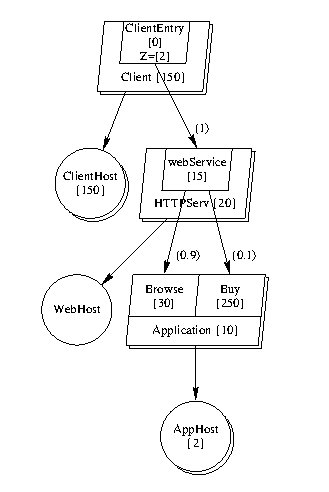
\includegraphics{model/notation.eps}
  \caption{A layered application with software and hardware servers.}
  \label{fig:notation}
\end{figure}

Figure~\ref{fig:notation} shows one graphical LQN notation. The tasks\index{task} (software servers)\index{server!software} are the
large parallelograms, and their entries are the enclosed parallelograms. The task of Figure~\ref{fig:elements} could for
instance be the \texttt{HTTPServ} task, with its thread pool indicated by the multiplicity\index{multiplicity} notation $m=20$\index{m@\texttt{m}}
for a limit of 20 threads. One \texttt{webService} request requires a total of 15 ms (CPU time) to
handle it, including receiving the request, interpreting it, and making a nested request\index{request!nested} to the
\texttt{Application}, receiving the response, and sending the final response page back to the
client. The pool of 150 clients is represented by the single \texttt{Client} task symbol, with an entry\index{entry}
that represents one cycle of client activity: think\index{think time} for 2 seconds, make one request. It runs on
a single processor. The request arrows to the \texttt{Application} entries show that 90\% of requests
are to the \texttt{Browse} entry, and 10\% to the \texttt{Buy} entry. The host demand\index{demand} of the entries is 30 ms for
\texttt{Browse}, 250 ms for \texttt{Buy}, and \texttt{Application} has 10 threads and runs on two cores (or a two-CPU
multiprocessor\index{multiprocessor}). The host demand labels indicate only one phase of service at each layer in
this model.

A real system may have additional layers. If this is an e-commerce system, the \texttt{Application}
will make requests to one or more database systems (which will in turn use a storage system), and
to some kind of financial server for the purchase transaction. An HTTP server usually has separate
storage for fixed page elements and makes requests to that.

\subsubsection{Tasks, entries, calls, demands}
\label{sec:tasks-entries-calls-demands}

The notation\index{notation} for layered queueing models uses the terms task\index{task}, host processor\index{processor}, entry\index{entry}, call\index{call}, 
and demand\index{demand}, as follows.

\begin{itemize}
\item \emph{Tasks}\index{task} are the interacting entities in the model. Tasks carry out operations defined by their \emph{entries}\index{entry}
  and also have the properties of resources, including a queue\index{queue!discipline}, a discipline, and a multiplicity\index{multiplicity}. A
  single-threaded task is itself a critical section\index{critical section}.

  Tasks that do not receive any requests are special; they are called \emph{reference tasks}\index{task!reference}\index{reference task} and represent
  load generators or users of the system, that cycle endlessly and create requests to other tasks. 
  Separate classes of users are modelled by separate reference tasks.
  
\item A task\index{task} has a \emph{host processor}\index{processor}, which models the physical entity that carries out the operations. 
  This separates the logic of an operation from its physical execution. The processor has a queue\index{queue!processor}\index{queue!discipline}
  and a discipline for executing its tasks, and a task has a priority\index{priority}. The host processor has a speed
  ratio relative to a ``standard processor'', such that when the host demand\index{demand} \emph{s} of an entry given for
  the standard processor, and the actual demand is $s$/(speed ratio)\index{speed ratio}.

  Thus a disk\index{disk} is modeled by two entities, a disk task representing the logic of disk operations
  (including the difference between say a read and a write, and the logic of disk device-level
  caching), and a disk device. 

\item \emph{Calls}\index{call} are requests\index{request} for service from one entry\index{entry} to an entry of another task\index{task}. A call may be 
  synchronous\index{call!synchronous}, asynchronous\index{call!asynchronous}, or forwarding\index{call!forwarding}\index{forwarding}, as discussed in Section~\ref{sec:calls}. This gives a rich 
  vocabulary of parallel and concurrent operations, expressed in a manner very close to that of a 
  software architecture\index{software architecture} description language. 

\item \emph{Demands}\index{demand} are the total average amounts of host processing and average number of calls for 
  service operations required to complete an entry. More detailed descriptions, detailing the 
  sequence of operations, can be given by giving the \emph{activity structure}\index{activity} of an entry\index{entry} or a
  task\index{task}, which will be described below.  
\end{itemize}

The basic use of these elements to model software tasks is illustrated in Figure~\ref{fig:notation}. Extensions of the
modeling concepts will be described later, including: defining parallel operations\index{parallel operations}\index{operations!parallel} with activities\index{activity},
using a task to model pure delays (such as a network latency), using a task to model other kinds of
software resources such as semaphores\index{semaphore}, exclusive locks\index{lock}, or buffer pools, and using forwarding\index{forwarding}
interactions to model asynchronous operations\index{operations!asynchronous}. A large family of replicated\index{replication} systems can be modeled
compactly using replication.

\subsection{Model workload parameters}

The software workload\index{workload} is described by the parameters of an activity\index{activity}. The basic model of an
entry\index{entry} assumes it has a single activity (sometimes called ``phase one''\index{phase!one} above); some systems have a
second activity (phase two\index{phase!two})\index{phase!two} after sending a reply. More generally, a graph of activities may be defined
to describe the execution of an operation (see section~\ref{sec:activities}). The parameters of an activity are:
\begin{itemize}
\item execution demand\index{demand}: the time demand on the CPU or other device (indicated by the parameter
labelled ``\parameter{s}'' in the modeling code)
\item wait delay (also called a \emph{think time}\index{think time}) (optional... it can be used to model any pure delay that does
not occupy the processor) (parameter label is ``\parameter{Z}'')
\item mean synchronous requests\index{request!synchronous} to another entry (token label is ``\parameter{y}'')
\item mean asynchronous requests\index{request!asynchronous} to another entry (parameter label is ``\parameter{z}'')
\end{itemize}
Additional optional parameters of an activity are:
\begin{itemize}
\item the probability of forwarding\index{forwarding}\index{call!forwarding} the request to another entry\index{entry}, rather than replying to it, when serving
a synchronous\index{request!synchronous} request (parameter label is ``\parameter{F}'', there can be multiple probabilities)
\item the squared coefficient of variation\index{squared coefficient of variation} of the execution demand requests. This is the ratio of the
variance\index{variance} to the square of the mean; for a deterministic\index{demand!deterministic}  demand its value is 0 (parameter label is ``\parameter{c}'')
\item a binary parameter to identify a \emph{stochastic sequence}\index{sequence!stochastic} in which the number of requests from the
activity is random, with a geometric distribution and the stated mean, versus a \emph{deterministic
sequence}\index{sequence!stochastic} in which the number is exactly the stated number (which must be an integer). (the
parameter label is ``\parameter{f}'', with value 0 for stochastic (the default) or 1 for a deterministic sequence)
\end{itemize}

\subsection{Performance measures: service time and utilization of an entry or a task}

The \emph{service time}\index{service time}\index{entry} of an entry, shown in Figure~\ref{fig:service-time}, is the time it is busy, in response to a single request. It includes
its execution time\index{execution time} and all the time it spends blocked, waiting for its processor and for nested lower\index{service!nested}
services to complete. The service time in a layered model is a result rather than a parameter, except
for pure servers\index{server!pure} such as hosts\index{host}.

\begin{figure}
  \centering
  \subfloat{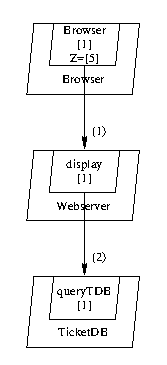
\includegraphics{model/service-time.eps}}\qquad
  \subfloat{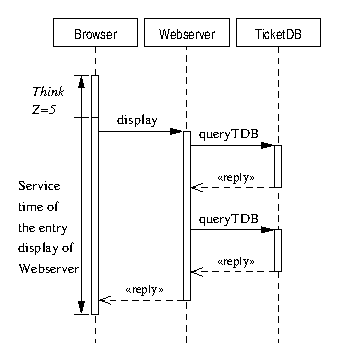
\includegraphics{model/service-time-seq.eps}}
  \caption{Service time of an entry\index{service time}, indicated on a sequence diagram.}
  \label{fig:service-time}
\end{figure}

Since a task\index{task} may have entries\index{entry} with different service times, the entries define different classes\index{service!classes}
of service by the task. The overall mean service time of a task is the average of the entry service
times (weighted by frequency of invocation).

The \emph{utilization}\index{utilization} of a single-threaded task is the fraction of time the task is busy (executing or
blocked), meaning not idle. A multi-threaded or infinite-threaded task may have several services
under way at once and its utilization is the mean number of busy threads\index{thread!busy}.

A saturated task\index{task!saturated} has all its threads busy almost all the time.

\subsubsection{Software Bottlenecks}

When a task\index{task} is fully utilized but the resources it uses (by nested calls\index{call!nested}, or its processor) are not
fully utilized, the task is called a ``software bottleneck''\index{bottleneck!software}\index{software!bottleneck}. A typical example is a single-threaded task
which blocks for I/O, and the typical cure is to multi-thread the task. Then when one thread is
blocked another one can proceed. (See the paper~\cite{perf:franks-2006-qest-bottlenecks} on software bottlenecks).

\section{Tools: the LQNS solver, the simulator, and their modeling language}
\label{sec:tools}

There are two solvers for layered queues, that take the same input files:
\begin{itemize}
\item The analytic solver \emph{lqns}\index{lqns} can be executed with the command line:
\begin{verbatim}
    lqns infile.lqn
\end{verbatim}
  (where the suffix \texttt{.lqn} is suggested, but not
  mandatory)\footnote{Input files with suffixes of \texttt{.lqn},
    \texttt{.in} or \texttt{.txt} are processed using the original
    input grammar.  All other suffixes are treated as XML input.} and it
  produces an output file with the default name \texttt{infile.out}. There are
  many options, which can be listed by invoking \texttt{lqns -h}. The
  documentation is the manual (``man'') page, also available in ASCII as
  \href{http://www.sce.carleton.ca/rads/lqns/lqn-documentation/lqns.txt}{\texttt{lqns.txt}}
  or PDF as \href{http://www.sce.carleton.ca/rads/lqns/lqn-documentation/lqns.pdf}{\texttt{lqns.pdf}}

The simulator \emph{lqsim}]\index{simulator}\index{lqsim} is invoked as:
\begin{verbatim}
   lqsim [run controls] infile.lqn
\end{verbatim}
and also generates an output file \texttt{infile.out}, which includes
confidence intervals on the estimated performance parameters.
Documentation is the man page for lqsim, the ASCII version
\href{http://www.sce.carleton.ca/rads/lqns/lqn-documentation/lqns.txt}{lqsim.txt},
or PDF as
\href{http://www.sce.carleton.ca/rads/lqns/lqn-documentation/lqns.pdf}{lqsim.pdf}
\end{itemize}

There are also two languages\index{model language}\index{XML} for defining models, a cryptic ``original'' language and an XML-based
language LQML\index{LQML} which is now the normative language. A conversion program \texttt{lqn2xml}\index{lqn2xml} is
used to convert between them. Since LQML is very verbose, models are often written in the original
language and converted before running, or run from that. Another approach is to use the semigraphical
editor jLQNDef\index{jLQNDef}\index{editor}. This editor can be used from scratch or to display and edit models
created earlier, and it can read and write in either syntax.

LQNS includes an experiment control\index{experiment control} section written in a language called LQX\index{LQX} (for LQ
eXperiments) which can set parameters to various values, extract and format results, and force new
solutions based on the results of a previous solution. LQX can only be
used with LQML input.

Simple experiments involving solutions over sets of parameter values can also be run with
LQNS/LQSIM in a simpler format using the ``original'' language\index{model language} plus annotations for parameters
and results. This facility replaces the experiment controller SPEX\index{SPEX}, which worked with the original
language but has become unmaintainable. See section~\ref{sec:spex}.

\subsection{XML Input File Grammar}
%\subsection{Model solver code for the reservation system in Figure~\protect{\ref{fig:ticket-reservation-system}}}
\label{sec:xml-grammar}

Input to the lqns model solver uses the schema shown in
Figure~\ref{fig:schema} on page~\pageref{fig:schema}\index{schema}.  The ``classes''\index{schema!classes} in
Figure~\ref{fig:schema} correspond to elements\index{schema!elements} in the XML input file.
The attributes\index{schema!attribtues} for the classes correspond to the most commonly used
parameters\index{XML!parameters} for a model.  Notice how every task must have a processor\index{processor},
and tasks\index{task} are used to model many things: devices other than CPUs,
external services that introduce a delay, users and their reaction
time, critical sections and locks, buffers, etc.

The behaviour of a task can be specified either using phases\index{phase} for an
entry\index{entry}, or through activities\index{activity} defined for a task.  Usually, it is
simpler to specifiy behaviour using phases (shown in black) since most
tasks do not incorporate internal parallelism.  The file
\texttt{reserv-templ} in the
Appendix~\ref{sec:reserve-templ} contains the reservation system.
It is a sample template file for models based entirely on entries.
More information about tasks modeled using activities is found in
Section~\ref{sec:activities}. 

\section{Task resources, queueing, and multiplicity (threads)}
\label{sec:tasks}

A task\index{task} models those properties of a software object which govern contention for executing the
object; it is identified with a \emph{task resource}\index{resource}, and a task queue\index{queue}. One task queue is used by all requests
to all the task's entries\index{entry}. Typically the software object is an operating system process, but tasks can
also represent other objects.

A \emph{single-threaded}\index{task!single-threaded} task can respond to one request at a time. A \emph{multi-threaded}\index{task!multi-threaded} task has a
limited pool of instances, each of which can respond to a request (it acts as a queueing multiserver\index{multiserver}).
The instances are homogeneous and are dispatched from a single queue, like any multiserver.
Multiple instances may be provided in different ways, for instance by process forking, by a static
pool of lightweight threads\index{thread} or kernel threads, or by re-entrant procedure calls. A special case which
can be modelled as multiple instances is a single carefully written process that accepts all requests,
and saves the context of uncompleted requests in data tables (this is called \emph{virtual threading}, or \emph{data
threading})\index{thread!data}\index{thread!virtual}

Some software objects are fully re-entrant and can exist in any number of copies, each with its
own context. These are often called multi-threaded, however because there is no limit to the number
of threads we will term them \emph{infinite-threaded}\index{thread!infinite}. They impose no resource constraint, and are used to
represent pure delays\index{delay}.

Multiplicity also applies to processors\index{processor} (hardware servers)\index{server!hardware} which may be defined as single,
multiple, or infinite. An infinite processor is an artificial entity introduced to provide a host for an
infinite task (every task must have a host\index{host}). If there are several infinite tasks, they can all be hosted
on a single infinite processor.

\subsection{Driver tasks and arrival processes}
\label{sec:driver-tasks}

Arrivals to the system are modeled by tasks which generate requests spontaneously, called
\emph{reference tasks}\index{reference task}\index{task!reference} in LQN. Any task with no requests made to it is a reference task. It should have a 
single entry with just one phase. Each reference task generates a separate class\index{class} of requests.

A closed class\index{class!closed} with population $N$ and think time $Z$ is represented by a reference task with
multiplicity\index{multiplicity} $N$ and think time\index{think time} $Z$, hosted by a processor with multiplicity at least $N$, and making 
synchronous requests\index{request!synchronous} (that block waiting for a reply). The importance of the blocking\index{blocking} is that the
client task cannot do anything else while the response is coming back, thus imposing the finite
population of simultaneous requests.

It is usually preferable to model open arrivals\index{class!open}\index{open arrival} by a closed arrival approximation (see below)
However, an open class with arrivals at rate f/sec can be modeled by a reference task\index{reference task}\index{task!reference} of multiplicity 
1 and think time\index{think time} $Z = 1/f$ sec, and making an asynchronous call\index{call!asynchronous} to some operation. Since the call is
asynchronous, the task immediately begins to generate the next call, giving the arrival process. If
the think time is exponentially distributed (the default), and the entry has a single deterministic
phase, the arrivals will be Poisson\index{Poisson arrival}. As an alternative way to model open arrivals, any entry can be
defined to have a Poisson stream of arrivals coming to it, in addition to other requests.

\subsubsection{Closed modeling of open arrivals}
Since the service time of entries in layered queueing is not 
known in advance (it may include lower-layer contention delays), it is not possible to guarantee that 
a given arrival rate does not over-saturate the system. The analytic solver and simulator detects this condition
during iteration and stops. For this reason it is better to make a closed approximation\index{close approximation} to the open stream. Introduce
a reference task\index{task!reference}\index{reference task} with a very large population $N$ (large relative to the expected queue lengths), and 
a large think time\index{think time} $Z = N/f$, to get an approximate rate $f$. If $N$ is not large enough, the rate will fall, and 
this is a signal to increase $N$ (or, that the system cannot handle the rate $f$/sec).

\subsection{Pseudo-tasks}
\label{sec:pseudo-tasks}

Artificial pseudo-tasks\index{task!pseudo} can be used to model a variety of things, including an internal
operation of a ``task'', a network delay\index{delay!network}, or a response-time measurement probe. They may be hosted
on pseudo-processors\index{processor!pseudo}.

\begin{figure}
  \centering
  \subfloat[a shared module]{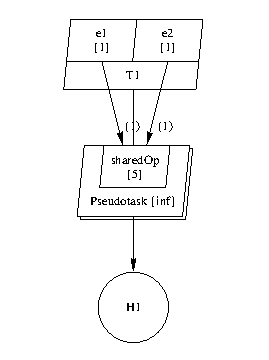
\includegraphics{pseudo-tasks/shared-module.eps}\label{fig:shared-module}}\quad
  \subfloat[a network latency]{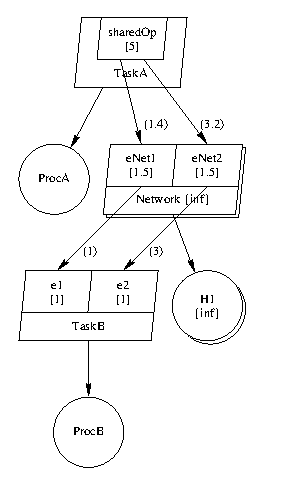
\includegraphics{pseudo-tasks/network-latency.eps}\label{fig:latency}}\quad
  \subfloat[instrumentation]{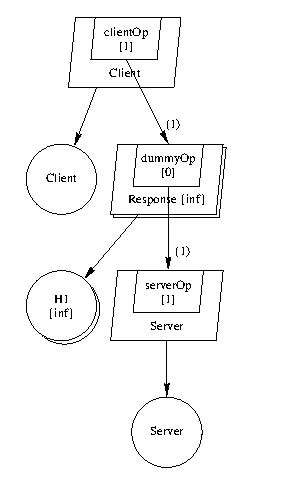
\includegraphics{pseudo-tasks/instrumentation.eps}\label{fig:instrumentation}}\quad
  \caption{Pseudotasks}
  \label{fig:pseudotasks}
\end{figure}

\subsubsection{An internal operation of a task}  
Refer to Figure~\ref{fig:shared-module}. A LQN task\index{task!internal operation} \texttt{T2} can model a re-entrant
module that has no attached resource significance, for example a module within a task \texttt{T1} that is
shared by several of its entries. Instead of including the workload of the module in all the entries, it
can be modelled separately (to better reflect the software structure, or just to calculate its loading
within the model). The pseudo-task\index{task!pseudo} \texttt{T2} is an infinite server\index{server!infinite} that runs on the same host as the task
\texttt{T1}. Since it is always called by an entry of \texttt{T1}, its task resources are provided by \texttt{T1}.

\subsubsection{A network delay}
Refer to Figure~\ref{fig:latency}. An infinite task\index{task!infinite} with host demand equal to the delay
time can be interposed in any call to impose this delay on the call. Multiple calls over the same
network to different destination entries must have separate entries in the delay pseudotask, to
separate the call routing. The task is hosted on an infinite pseudo-processor of speed factor 1.0.

\subsubsection{Response-time instrumentation} 
Refer to~\ref{fig:instrumentation}. The LQNS solver returns the delay to a
call (such as the call from \texttt{clientOp} to \texttt{serverOp} in Figure~\ref{fig:instrumentation}) in two parts, as the queueing time of
the request at \texttt{Server}, plus the service time\index{service time} of the entry \texttt{serverOp}. Purely for convenience, we
sometimes define a dummy pseudotask that simply passes on the call; the task ``Response'' blocks
for a time equal to the queueing plus service at serverOp. ``Response'' does not have to be infinite,
but it and its pseudo-processor\index{processor!pseudo} host must have equal or greater multiplicity, than \texttt{Client.}

\section{Styles of interaction}
\label{sec:calls}

We can model three kinds of interactions between entries\index{entry} which are
illustrated by a sequence diagram in Figure~\ref{fig:calls-seq}
matching the LQN diagram in Figure~\ref{fig:calls} for each interaction.

\begin{figure}[htbp]
  \centering
  \subfloat[Nested synchronous calls]{
    \hspace{0.25cm}
    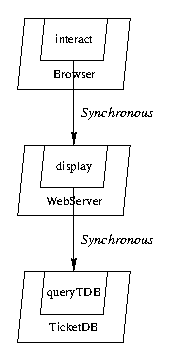
\includegraphics{calls/rnv.eps}
    \hspace{0.25cm}
    }\hspace{0.5cm}
  \subfloat[Forwarded query, replying directly to the client]{
    \hspace{0.25cm}
    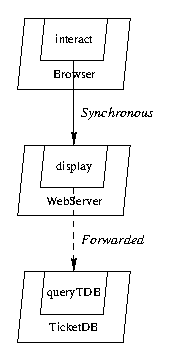
\includegraphics{calls/fwd.eps}
    \hspace{0.25cm}
    }\hspace{0.5cm}
  \subfloat[External arrivals, and an asynchronous invocation]{
    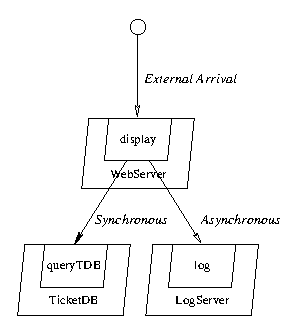
\includegraphics{calls/snr.eps}
    }
  \caption{Layered Queueing notation for the three styles of interaction.} 
  \label{fig:calls}
\end{figure}
\begin{figure}[htbp]
  \centering
  \subfloat[Nested synchronous calls]{
    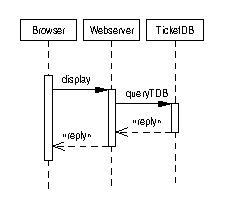
\includegraphics[scale=1.2]{calls/rnv-seq.eps}
    }\hspace{1cm}
  \subfloat[Forwarded query, replying directly to the client]{
    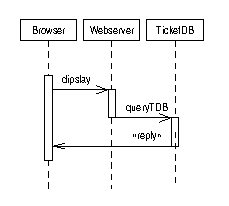
\includegraphics[scale=1.2]{calls/fwd-seq.eps}
    }\hspace{1cm}
  \subfloat[External arrivals, and an asynchronous invocation]{
    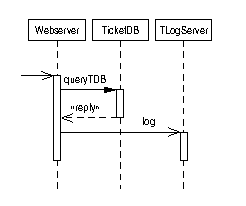
\includegraphics[scale=1.2]{calls/snr-seq.eps}
    }
  \caption{UML Sequence Diagrams showing the messages passed. In this
  notation, the solid arrowhead shows a synchronous message, with a
  dashed arrow for the reply.} 
  \label{fig:calls-seq}
\end{figure}
\begin{itemize}
\item \emph{asynchronous call:}\index{call!asynchronous} the sender does not wait and receives no
  reply. The receiving entry operates autonomously and handles the
  request. 

  This propagates the workload among the servers and gives the resource utilizations and
  throughputs, but it is an effort to determine the delays along the path taken by a request. For this
  reason an asynchronous chain of operations may be modeled by forwarding\index{forwarding}.

\item \emph{synchronous call}\index{call!synchronous}, with a reply\index{reply}: The sender waits
  (blocked) for the reply, and the receiving entry must provide
  replies. This is the pattern of a standard remote procedure call\index{remote procedure call}
  (RPC). The sending object task resource or thread is regarded as
  busy during the wait.
  
  For non-blocking software the request-reply structure may be kept in the model by introducing
  artificial sender threads\index{thread}, one for each potential outstanding reply. In the model these threads do
  block and wait for the reply, and they accumulate the total time to complete a response. These
  threads need not exist explicitly in the software.

  Some ``delayed-synchronous'' interactions with a reply actually continue in parallel\index{server!parallel} with the
  execution of the server, and later attempt to pick up the reply from an agent or mailbox. This can
  be modeled as parallel execution, with activities\index{activity} (see section~\ref{sec:6}).

\item \emph{forwarding interaction:}\index{forwarding}\index{call!forwarding} the first sender sees a synchronous
  interaction, and waits for a reply. However the receiver does not
  reply, but rather forwards the request to a third party, which
  either replies, or forwards it further. This gives an asynchronous
  chain of operations for a waiting client.  Further, at each step there may multiple forwarding targets, with probabilities.

  Asynchronous sequences\index{sequence!asynchronous} of events can be modeled by forwarding\index{forwarding}, in order to structure the
  sequences in the model and to capture the delay over a path. If the sender does not block, an
  instrumentation pseudotask\index{task!pseudo} (infinite-threaded) can be introduced to at the beginning of the path,
  which forwards the request, receives the final ``reply'' when the sequence ends, and records the
  delay as the service time of the waiting thread.
\end{itemize}

\section{Adding detail with activities within an entry}
\label{sec:activities}
\label{sec:6}

The simplest operation by an entry is a single activity\index{activity}, followed by a reply\index{reply} to the invocation.
However it is important to be able to specify more complex behaviour patterns, including 
operations in a particular sequence, and parallel subthreads\index{thread!parallel}. This is done by specifying a precedence 
graph\index{precedence graph} of activities, starting from the first activity for the entry\index{entry}.

Each activity is described by a set of parameters with labels ``\parameter{s}'', ``\parameter{y}'', ``\parameter{f}'', ``\parameter{c}'' etc., as described in
Section~\ref{sec:tasks-entries-calls-demands}. The graph can then be described by a series of textually specified relationships: 

\begin{tabular}{lp{2.5in}p{2in}}
\hline
Sequence\index{sequence}\index{->@\texttt{->}}: & \verb!a1 -> a2! & activity 1 preceedes activity 2 \\
AND-fork\index{fork!AND}\index{AND-fork}\index{->@\texttt{\&}}: & \verb!a1 -> a2 & a3! &  activity 1 precedes activities 2, 3...
in parallel (an AND-list of any length) \\
AND-join\index{join!AND}\index{AND-join}: & \verb!a1 & a2 -> a3! &  predecessors are an AND-list of any length. \\
OR-fork (branch)\index{fork!OR}\index{OR-fork}\index{branch}\index{->@\texttt{+}}: & \verb!a1 -> (p2) a2 + (p3) a3! & \\ 
OR-join (merge):\index{join!OR}\index{OR-join}\index{merge} & \verb!a1 + a2 -> a3! & predecessors may be an OR-list of any length. \\ 
LOOP\index{LOOP}\index{->@\texttt{*}}: & \verb!a1 -> n2 * a2,  n3 * a3, a4! & a repeated activity 2, and a repeated activity 3,
followed by activity 4.\\ 
\hline
\end{tabular}

If the repeated part is not a single activity\index{activity} then:
\begin{itemize}
\item if it is a sequence, the rest of the sequence is defined separately, with a definition that it is
  preceded by activity1.
\item If it is a complex structure of activities it can be packaged into a separate pseudo-task\index{task!pseudo} (as
  described in Section 2.1), called by activity1. This pseudo-task can contain forks\index{fork} and joins\index{join} and
  other behaviour structure nested within the loop.
\end{itemize}

Figure~\ref{fig:activities} shows an example, including both ways to structure a loop\index{loop}. 
The reply is sent after \texttt{a10}. The loop defined by the call from \texttt{a14} is defined in the workload
parameters of \texttt{a13}, not in the precedence graph\index{precedence graph}. The parallel activities \texttt{a7} and \texttt{a8} are executed by
two concurrent threads\index{thread!concurrent} which compete for the host processor; one or both are assumed to be created
dynamically at the fork and destroyed at the join. Physical parallelism\index{parallelism} is obtained when the host is a
multiprocessor\index{processor}, or if one or both of these activities call other tasks on different hosts. 

\begin{figure}[htbp]
  \centering
  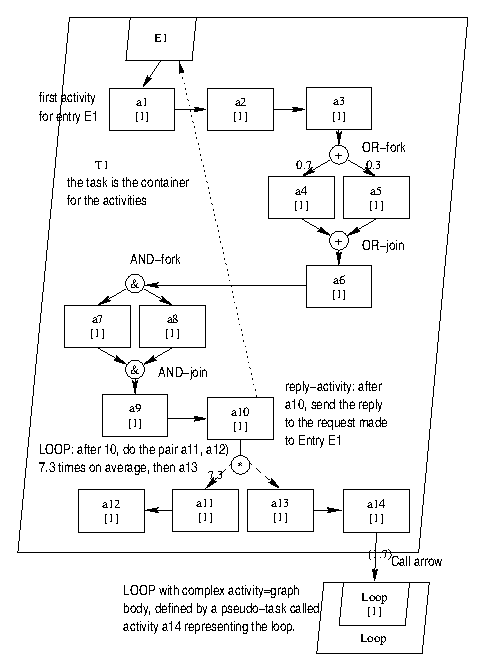
\includegraphics{model/activity-model.eps}
  \caption{Task with activities}
  \label{fig:activities}
\end{figure}

Although there is commonly a separate sub-graph for each entry, the activity graph is a
property of the task as a whole. The reason is, that it allows one to define a single graph with
multiple starting points at two or several entries, for instance to define a task which joins flows from
two different tasks. 

Parallelism\index{parallelism} in layered queues is discussed in~\cite{WOSP98:franks-98}.

\subsection{LQN code for the activity section}
\label{sec:activities-code}

LQN code for the activity section The textual definition above is part of the ``original'' LQN language; the XML-based LQML
has a more extended syntax.

In the LQN language, the entries which use activities are identified in the entry list, along
with the first activity in the entry. In a separate activity section for the task, the workload
parameters of the activities and their precedence relationships are defined for all the entries that
have activities. Also the workload of each activity is defined, using the parameters defined in
Section 3.1. The template file \texttt{activity-templ.lqn}, repesenting a server with OR and AND
forks, is commented to document the 
syntax including that for activities.

\subsection{Modeling Asynchronous RPC, and Prefetching}
\label{sec:asynch-rpc}


An asynchronous RPC\index{remote procedure call!asynchronus} is modeled by forking\index{fork}\index{activity} an 
activity to make the RPC, and joining at the point where the result is picked up by the main flow.
Prefetches\index{prefetch} are modeled similarly, as are ``futures'' operations (which do a speculative computation\index{speculative computation}
in parallel). 

\section{Service with a Second Phase}
\label{sec:second-phase}

A wide variety of software services give a reply to the requester
before they are entirely finished, in order to release the requester
from the synchronous call\index{call!synchronous} delay as soon as possible. The remaining
operations after the reply\index{reply} are done under sole control of the server
task, and they form the second phase\index{phase!second}. This behaviour is shown in
Figure~\ref{fig:second-phase}.  A special shorthand is used to
represent this common case.

\begin{figure}[htbp]
  \centering
  \subfloat[Behaviour]{
    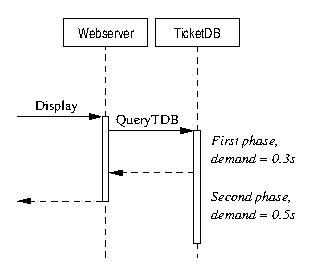
\includegraphics{model/phase-seq.eps}
}
  \subfloat[LQN with phases in TktD ]{
    \hspace{1cm}
    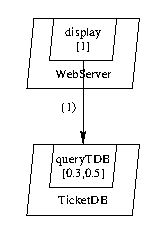
\includegraphics{model/phase-entry.eps}
    \hspace{1cm}
}
  \subfloat[LQN with activities in TktDB (activities shaded)]{
    \hspace{1cm}
    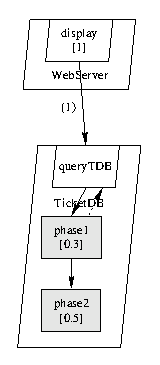
\includegraphics{model/phase-activity.eps}
    \hspace{1cm}
}
  \caption{A second phase of service lets the client of the interaction proceed}
  \label{fig:second-phase}
\end{figure}

Entries\index{entry} with phase one\index{phase!one} and phase two\index{phase!two}a can be represented by two
activities\index{activity!phase}, one performed before the reply\index{reply} and one after. Because they
all have this simple structure they can be defined directly for the
entry, without an explicit precedence graph. Each entry has a vector
for each workload parameter, with a value for each phase. Thus the
execution demand for the entry \texttt{queryTDB} above would be defined by a
line beginning with code "s" for execution demand:  
\begin{verbatim}
  s queryTDB 0.3 0.5 -1
\end{verbatim}
The host demands\index{demand} are 0.3 for phase one\index{phase!one}, 0.5 for phase two\index{phase!two}. Note that the
separator \texttt{-1}\index{-1@\texttt{-1}} is used in many places in the definition language.

Second phases\index{phase!second} are common. An example is seen in a write operation to
the Linux NFS file server; the write operation returns to the
requester once the file is buffered in the server, and the actual
write to disk is performed later, under sole control of the server.
Doing the writes in first phase would be safer, because the client
would be told if the write failed, and this is how the NFS protocol
was originally defined. Other NFS implementations allow second-phase
or delayed writes only if the server has a battery-powered buffer to
provide security of the data, in case of a power failure.

Second phases improve performance\index{performance!second phase}; they give less delay to the client,
and they increase capacity because there can be some parallel
operation between the client and the server. The amount of gain
depends on circumstances (real parallelism\index{parallelism} needs separate processors,
and a saturated server cannot increase its capacity).

The extreme case of all execution being in second phase is a kind of
acknowledged hand-over of data from the client to the server. Thus it
is similar to an asynchronous message\index{call!asynchronous}, except that the sender waits
for the acknowledgment. One important advantage of this is that the
sender cannot over-run the receiver; the sender is throttled by the
waiting for acknowledgments.

\subsubsection{Results for second phase at a single server, and at two layered
servers}

If some of a task's work can be put into the second phase, the task
can return more quickly to its clients. However if the task is already
saturated the clients have to wait for many other services anyway and
the advantage is small or even nil. The degree of improvement thus
depends on the degree of saturation, and where the saturation is.
Table~\ref{tab:second-phase} shows how a group of users with a 5-sec
thinking time are affected when the server service time is split
between phase one\index{phase!one} and phase two\index{phase!two} in different ratios (LQNS approximate
results). At low utilizations\index{utilization}, more phase two\index{phase!two} is uniformly better, but
as utilization increases, the best split moves towards the middle.

\begin{table}[htbp]
  \centering
  \begin{tabular}{|c|*{6}{d{5}|}}
    \hline
    nusers 
    & \multicolumn{6}{c|}{Response time (sec) for different values of demand s = [phase 1, phase 2]} \\
    \cline{2-7}
    & \multicolumn{1}{c|}{s = [0,1.0]}
    & \multicolumn{1}{c|}{[0.2,0.8]}
    & \multicolumn{1}{c|}{[0.4,0.6]}
    & \multicolumn{1}{c|}{[0.6,0.4]} 
    & \multicolumn{1}{c|}{[0.8,0.2]}
    & \multicolumn{1}{c|}{[1.0,0]} \\  
    \hline
    1      &  0.166     & 0.310     & 0.464   &  0.629   &  0.807   &  0.999   \\
    4      &  1.125     & 0.726     & 0.827   &  0.996   &  1.269   &  1.6420  \\
    7      &  3.066     & 2.694     & 1.5087  &  1.7928  &  2.269   &  2.9256  \\
    10     &  4.8474    & 4.2741    & 3.8951  &  3.98149 &  4.4927  &  5.221   \\
    15     &  9.9096    & 9.4738    & 9.2281  &  9.2289  &  9.5048  &  10.037  \\
    20     &  14.9381   & 14.541    & 14.323  &  14.318  &  14.548  &  15.0120 \\
    \hline
  \end{tabular}                                             
  \caption{The impact of dividing a unit server demand between phase 1 and phase 2}
  \label{tab:second-phase}
\end{table}


\section{Logical resources (critical sections, locks, buffers)}
\label{sec:logical-resources}

The task\index{task} entity in layered modeling is used to model any resource whatever. Consider first a
critical section\index{critical section} shared by a set of concurrent threads or processes. There are two cases:
\begin{itemize}
\item if the threads or processes are on the same processor, and they all execute the identical operation
  in the critical section (this is like a monitor\index{monitor}) then the operation can be removed from the tasks
  and made into an entry in a pseudo-task\index{task!pseudo} with multiplicity 1. This is like a pseudo task for an
  internal operation, but imposing concurrency restrictions.
\item if the threads or processes are on different hosts, or they execute different operations in the
  critical section, then the pseudo-task with multiplicity 1 runs on a psedo-processor, with an
  entry for each caller... this entry calls a sort of shadow task\index{task!shadow} defined for each process, which
  represents the critical section\index{critical section} workload of that process. The shadow tasks are defined as a ``task
  for an internal operation'' described above, with multiplicity 1, and run on the same host as the
  caller. Only one of these shadow tasks can be active at once, and a queue of requests forms
  before the critical section ``task''. Effectively the calling tasks are split into a task for the
  workload outside the critical section, and a task for the inside.
\end{itemize}
The same approach can be applied to locking a table, with the operations applied while
holding the lock\index{lock}, treated as a critical section. A complex locking system, with many separate locks,
and read and write locks, requires special treatment. The queuing disciplines are complex, and there
are often too many locks to represent each one separately. This is a subject of current research.

Memory\index{memory} and buffer\index{finite buffer} resources can be modeled similarly, with a multiple ``task'' (the same
designation as a multi-threaded task\index{task!multi-threaded}) to represent the resource, and with entries to activate the
workload for each user.

\subsubsection{Modeling finite buffers:}
\label{sec:finite-buffers}

A finite buffer\index{finite buffer} space, which blocks its senders when it is full, can
be modeled by a multi-threaded buffer task with second-phase\index{phase!second}
interactions going into and coming out of the buffer.  The model is
shown in Figure~\ref{fig:finite-buffers}.  Each buffer space is
modeled by a \emph{``thread''}\index{thread} which immediately replies\index{reply} (releasing the sender)
and then sends to the receiver (and waits until the receiver replies,
to acknowledge receipt).

\begin{figure}[htbp]
  \centering
  \subfloat{
    \hspace{1cm}
    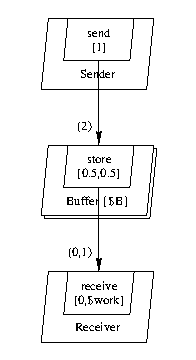
\includegraphics{model/buffer.eps}
    \hspace{1cm}
    }
  \subfloat{
    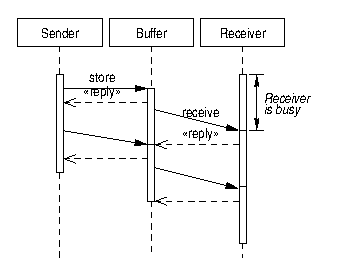
\includegraphics{model/buffer-seq.eps}
    }
  \caption{Buffer pseudo-task.} 
  \label{fig:finite-buffers}
\end{figure}


\section{Limitations}
\label{sec:limitations}

This is not a complete list, but notes some limitations\index{limitations} that have come
up:

\begin{itemize}
\item recursive calls\index{calls!recursive} are excluded (a task calling its own
  entries)... the approach for dealing with recursive calls is to
  aggregate the demand into the first entry. Possibly this should be
  accommodated, but it requires an assumption that the same thread
  handles the recursive request (to avoid deadlock when threads are
  limited), which limits the behaviour of an entry.
\item replication of subsystems\index{replication!subsystem} (without defining all the replicas
  separately) is handled but only with restrictions; a thesis is
  available~\cite{THESIS:pan-96}.
\item activity sequences which fork in one task and join in another can be solved by the simulation
  solver (lqsim)\index{simulation}.
\item external arrival flows may be specified into an entry, however a
  system with only external arrivals causes problems for the analytic
  solver. It is recommended to define sources of traffic as tasks
  which make requests and block; this has the advantage that it never
  overruns the system. Message loss is not modeled; current research
  may cure this.
\item exceptions\index{exceptions} and timeouts\index{timeouts} are also not modeled, similar comment.
\end{itemize}

\section{Reference material}
\label{sec:reference-material}

\begingroup
\renewcommand{\section}[2]{}
\bibliography{tutorial}
\endgroup

Also, see the web pages:

\begin{itemize}
\item \url{http://www.layeredqueues.org/} includes a bibliography on layered queueing.
\item \url{http://www.sce.carleton.ca/rads} for material on the larger project
  (RADS is the Real-time And Distributed Systems group at Carleton),
  and for software download. 
\item \url{http://www.sce.carleton.ca/rads/lqn/lqn-documentation}
\item \url{http://www.sce.carleton.ca/faculty/woodside} for my bibliography
  material.
\end{itemize}

\section{Running the tools}
\label{sec:execution}

LQNS is available from the \href{http://www.sce.carleton.ca/rads/lqns/LQNSDownload}{download page} (you will need to sign a license and fax it) for
Linux, Windows and MacOSX. It has a \href{http://www.sce.carleton.ca/rads/lqns/lqn-documentation/lqns.pdf}{comprehensive man page}
describing many options for different solver algorithms, for tracing solutions and for printing more
or less detail. The best reference on the many solver options is Greg Franks' PhD thesis~\cite{THESIS:franks-99}.

The LQNS input language is essentially documented by the comments in
the example files found ni the Appendicies.
There is a BNF definition included in the more extensive discussion of activity notation, in
``Parallel Activity Notation in LQNS'' by Franks (Chapter 6 in the thesis~\cite{THESIS:franks-99}). Personally I
create models starting with one of two template files that include example definitions and comments
defining the syntax. \texttt{template.lqn} does not include activities, \texttt{activity-template.lqn}
does. I replace the model in the template by the one I want.

LQML\index{LQML} is the more recent XML-based\index{XML} language, with \href{http://www.sce.carleton.ca/rads/lqns/lqn-schema/lqn.xsd''}{schema \texttt{lqn.xsd}} (and there are two
sub-schemas with it). You can convert between the two languages with the program \texttt{lqn2xml}\index{lqn2xml}, or the
\texttt{jlqndef} editor. If you need the XML it may be preferable to create the model in the input language
and convert, writing models in XML is brutal.

\texttt{lqn2ps}\index{lqn2ps} is a program for creating a graphical image in many formats, not just postscript.

\texttt{Jlqndef}\index{jlqnDef} is a graphical and text-window-based editor which shows a simple diagram of the
model. It requires Java 1.1.3 or higher, with the ``swing components''.

\subsection{Efficient experiment control}
\label{sec:spex}

Two ways are provided to do parameter sensitivity and other experiments under program
control, and extract the results in a compact form.
\begin{enumerate}
\item The most general is to write a progam in LQX\index{lqx} and include it in a LQML\index{LQML} definition file (see the
  LQNS User Guide~\cite{MANUAL:lqns})
\item A more restricted but useful capability allows one to define sets of values of parameters, and then
  evaluate models for all combinations of these values. This replaces SPEX\index{SPEX}. It is provided by \texttt{lqns}
  or \texttt{lqsim} using the original LQ language with SPEX-like additions to the model file, which are
  described in the User Guide. If you are familiar with SPEX, the main difference is that the
  parameter range definitions must be enclosed in square brackets (e.g. \verb!$param = [1,6,15,37]! or
  \verb!$param = [10:100,10]!. Also expressions\index{SPEX!expressions} must conform to LQX rather than PERL, comments must
  begin with \verb!#!, and string substitution is not supported, and there is a change to how solver pragmas
  are set.

  If you are not familiar with SPEX, a simplified description of experiment control\index{experiment control} follows (for more
  capabilities and details see the User Guide, section 5.3):
  \begin{itemize}
  \item before the model begins, add lines of form \verb!$paramname = [value1, value2,...]! or \verb!$paramname = [start:end,increment]! 
    (where \emph{paramname} must begin with \$) to define the experiment cases.
  \item optionally you can define other named parameters\index{parameters!named} as
    functions (expressions) of these, using \texttt{+}\index{+@\texttt{+}}, \texttt{-}\index{-@\texttt{-}}
    \texttt{*}\index{*@\texttt{*}}, \texttt{/}\index{/@\texttt{/}} and \texttt{**}\index{**@\texttt{**}} operators\index{operators} in the usual way.
  \item within the model, use \verb!$paramname! in place of the numeric model parameter value.
  \item add results definitions\index{result defintions} at the ends of lines defining processors, tasks, entry host demands and
    calls. Each result definition is of the form \verb!%X $resultname!, where \emph{resultname} also begins with \$
    and \texttt{X} is a code, one of:
    \begin{description}
    \item[\parameter{u}:] (utilization)\index{utilization}, 
    \item[\parameter{pu}:] (processor utilization)\index{utilization!processor},
    \item[\parameter{s0}:] (total entry service time)\index{service time}, 
    \item[\parameter{s1}:] (entry phase one service time), 
    \item[\parameter{s2}] (entry phase 2 service time), and
    \item[\parameter{f}:] (entry or task throughput)\index{throughput}.
    \end{description}
  \item after the model, add a section starting with ``\verb!R 0!''
    and ending with ``\verb!-1! with a list of items:
    \begin{enumerate}
    \item parameter names, 
    \item result names,
    \item \verb!$var = expression!,
    \end{enumerate}
    one per line with no end of line termination.   Each case solved will give one line of results with these values in the order defined.
    The special parameter \verb!$0!\index{\$0@\texttt{\$}} is the model number created by the solver, starting from one.
  \item The results from the solution will be directed to the terminal
    by default.  They can be redirected using ``\verb!-o!
    \emph{filename}''. 
  \end{itemize}
\end{enumerate}

\section{Questions}
\label{sec:questions}
\begin{itemize}
\item \emph{Throughput\index{throughput} refuses to increase when I introduce more
  resources.} Search for a saturated resource; it may represent a
  modeling error. For instance, if one introduces more users, one must
  also introduce more processors for them to run on. A simple
  expedient is to make any resource which should not be a limit,
  infinite. This is also solver-friendly, a infinite resources are
  easy. 
\item Convergence: \emph{what if my LQNS solution does not converge?} The
  symptom is that the convergence\index{convergence} value for the iterations is greater
  than the set value, typically $10^{-6}$. Sometimes, especially in
  heavily loaded systems, the iterative solver will cycle and not
  converge. One cure which is sometimes effective is to reduce the
  value of the under-relaxation\index{under-relaxation} coefficient in the solver controls,
  from a typical value of 0.9 or 0.7 to a low value, of say 0.1. This
  is intended to force convergence by reducing the step size. If this
  does not succeed, then as long as the convergence value is less than
  0.1, the solution found has some reasonable relationship to the
  correct value. (The size of the convergence value is the largest
  relative change from one iteration to the next, of any of the
  variables in the model; it does not directly indicate the size of
  errors, but if the solution is in fact cycling around the correct
  solution then all relative errors are probably smaller than this). A
  method which is usually not effective is to increase the number of
  iteration steps\index{iterations}. The basic recourse for greater accuracy is to
  simulate. 
\item Replication: \emph{how can I model a system with many repetitions of a
  subsystem within it?} Provided the replications\index{replication} are identical in
  every respect, and divide all their interactions with the rest of
  the system equally, the replication feature of LQNS can give
  efficient solutions. The full documentation of this feature is in
  the Master's thesis of Amy Pan. Briefly, any task can have a
  replication factor $r$, which means that multiple copies are
  created. If its processor has the same $r$, then each copy has a
  separate processor. If it communicates with other tasks with the
  same $r$, it communicates with just one of them, and the interactions
  are assumed to form $r$ subsystems. Messages between tasks with
  different $r$ must have values of fan-in ``\parameter{i}'' and fanout ``\parameter{``o''} such that
  the product of $\textrm{source~} (r \times \textrm{fanout}) = \textrm{destination~} (r \times
  \textrm{fan-in})$. These factors \parameter{i} and \parameter{o} describe the replication\index{replication!calls} of the
  message arcs. 
\item Odd results for multiple servers: \emph{if I run for a series of
    values of $m$ for server multiplicity, I may see rising throughput\index{throughput};
    then for $m=\infty$, the throughput drops a bit. How come?} The
  waiting time calculation for a multiserver\index{multiserver!approximation} is an approximation, and
  errors of a few percent are to be expected. The infinite server
  queue is solved exactly (no waiting). If the anomaly is worrying,
  try a more exact multiserver algorithm by using
    ``pragma~-Pmultiserver=conway'', but it will take longer. 
\item Non-blocking systems: \emph{in my model the servers are
  asynchronous. A server processes each message, whether a request or
  a reply, and then takes whatever message comes next. I never blocks
  to wait for a reply. How to model it?} Such a server is modeled with
  infinite threads\index{thread!infinite}, allowing one active thread for each uncompleted
  request it is processing. This may be called virtual threads\index{thread!virtual} or data
  threads\index{thread!data} , since the request context, if any, is managed by user
  data.
\item Solution Time: \emph{my LQNS solution takes a long time (a
    minute is long for a few tasks; 10 minutes is long for any
    model)}. Possible reasons are:
  \begin{enumerate}
  \item poor convergence\index{convergence} (see below)...
  you may want to reduce the iterations\index{iterations} or simulate;
\item a huge number
  of classes, generated by having a lot of separate source
  tasks\index{reference task} (``reference tasks'' and lots of entries on worker tasks.... you
  could get faster results if the sources were combined into fewer
  tasks, with random splits to generate the requests they make into
  the service layers.
\item do you have a multiserver (not a reference
  task) with a large m (say, $m> 20$?)... or layered multiservers one
  above the other, with moderate m... multiserver\index{multiserver!solution} solutions are only
  moderately expensive by the default algorithm, but the others cost
  more. You might consider whether it could as easily be infinite (if,
  say, its usage is well below the limit so the limit is not a
  factor). 
  \end{enumerate}
  In any of these cases, you might try to simulate\index{simulation}; there
  have been models that solved faster by simulation.
\item Cycles: \emph{what do I do if my model has a synchronous
    messaging cycle?} LQNS will refuse to solve a model, however it
  can be instructed to ignore the cycle checker with the
  \texttt{pragma~cycles=allow}\index{cycles!allow}. It then solves the model with an
  implicit assumption that if deadlocks\index{deadlock} are possible, they do not
  occur or are resolved.  The simulator (lqsim) will take a model
  with cycles at any time, however if a deadlock occurs as a result of
  a cycle, the simulation stops without any diagnostic.
\item Delay: \emph{how can I get the result for delay from an input at
    one point, to a response completion somewhere else in the model?}
  The cleanest approach is to introduce some special model elements:
  first, at the start of the response, introduce a pseudo-task R to
  capture the delay as its service time. It has zero demands (s = 0),
  has infinite multiplicity (code i) runs on its own processor or an
  infinite processor, has deterministic phases (f = 1) and makes one
  synchronous call to the input point to start the response. Second,
  create a forwarding chain through the model along the path of the
  response, so that the reply is created at the completion point; the
  reply goes back to the pseudo-task R, and ends its blocking state.
\item Simulation accuracy\index{simulation!accuracy}: \emph{how can I tell how accurate my
    simulation is?} It is essential to get confidence
  intervals\index{confidence intervals} out of
  the simulation. If you don't know about these, you will have to
  consult a statistics text. Lqsim will calculate confidence
  intervals for you, for all its results, if you run with the
  \texttt{-A} (automatic) or \texttt{-B} (batched) run options. These
  have the form -A,a,p,b or -B,n,b where b is a batch length in model
  time units, which should be say 100 times longer than the longest
  service time in your model, and n is the number batches (suggest 30,
  which is the max allowed). For A, a is the accuracy target in 5 of
  mean values, p is the confidence level.
\end{itemize}
\clearpage
\section{Model File: reserve-templ.lqn}
\label{sec:reserve-templ}
\lstset{basicstyle=\ttfamily\footnotesize,stringstyle=\emph,columns=fullflexible}
\lstset{keywordstyle=\color{blue},keywordstyle={[2]\color{red}}}
\lstinputlisting[language=LQN]{web-server/reserve-templ.lqn}
\clearpage
\section{Model File: activity-templ.lqn}
\label{activity-templ}
\lstinputlisting[language=LQN]{activity-templ/activity-templ.lqn}
\clearpage
\printindex
\end{document}
